\documentclass[tikz]{standalone}
% \usepackage{amsmath}
\usetikzlibrary{arrows,decorations.markings,fit,matrix,positioning,shapes}
\tikzset{
    % >=latex,
    mymatrix/.style={matrix of nodes, nodes=typetag, row sep=.2em},
    mycontainer/.style={draw=gray, inner sep=.1ex},
    typetag/.style={draw=gray, inner sep=1ex, anchor=west},
    title/.style={draw=none, color=gray, inner sep=0pt},
    arrowfwd/.style={decoration={markings,mark=at position 1 with {\arrow[scale=2,>=stealth]{>}}},postaction={decorate}},
    arrowboth/.style={decoration={markings,mark=at position 0.15 with {\arrow[scale=2,>=stealth]{<}},mark=at position 1 with {\arrow[scale=2,>=stealth]{>}}},postaction={decorate}},
    borderthick/.style={draw,draw=black!50,thick},
    recwht/.style={draw,minimum width=3cm,minimum height=2cm,align=center,text width=3cm,text=black,fill=white,draw=black!50,thick},
    recred/.style={draw,minimum width=3cm,minimum height=2cm,align=center,text width=3cm,text=black,fill=red!30,draw=black!50,thick},
    squorg/.style={draw,minimum width=2cm,minimum height=2cm,align=center,text width=2cm,text=orange,fill=white,draw=orange!50,thick},
    rndred/.style={rounded corners=1cm,draw,minimum width=3cm,minimum height=2cm,align=center,text width=3cm,text=red,fill=rwhite,draw=red!30,thick},
    rndyel/.style={rounded corners=1cm,draw,minimum width=3cm,minimum height=2cm,align=center,text width=3cm,text=yellow,fill=white,draw=yellow!50,thick},
    diared/.style={diamond,draw,minimum width=3cm,minimum height=2cm,align=center,text width=3cm,text=red,fill=white,draw=red!30,thick,aspect=1.5},
    diayel/.style={diamond,draw,minimum width=3cm,minimum height=2cm,align=center,text width=3cm,text=yellow,fill=white,draw=yellow!50,thick,aspect=1.5},
    cirblu/.style={circle,draw,minimum width=2cm,minimum height=2cm,align=center,text width=2cm,text=blue,fill=white,draw=blue!50,very thick},
    cirred/.style={circle,draw,minimum width=2cm,minimum height=2cm,align=center,text width=2cm,text={rgb:red,255;green,0;blue,122},fill=white,draw={rgb:red,255;green,0;blue,122},very thick},
    cirpur/.style={circle,draw,minimum width=2cm,minimum height=2cm,align=center,text width=2cm,text={rgb:red,130;green,60;blue,250},fill=white,draw={rgb:red,130;green,60;blue,250},very thick},
    cylwht/.style={cylinder,draw,shape aspect=.5,cylinder uses custom fill,cylinder end fill=white,minimum width=1cm,minimum height=1cm,cylinder body fill=white,opacity=1,scale=2,draw=black!50,thick,rotate=90}
}
\begin{document}
    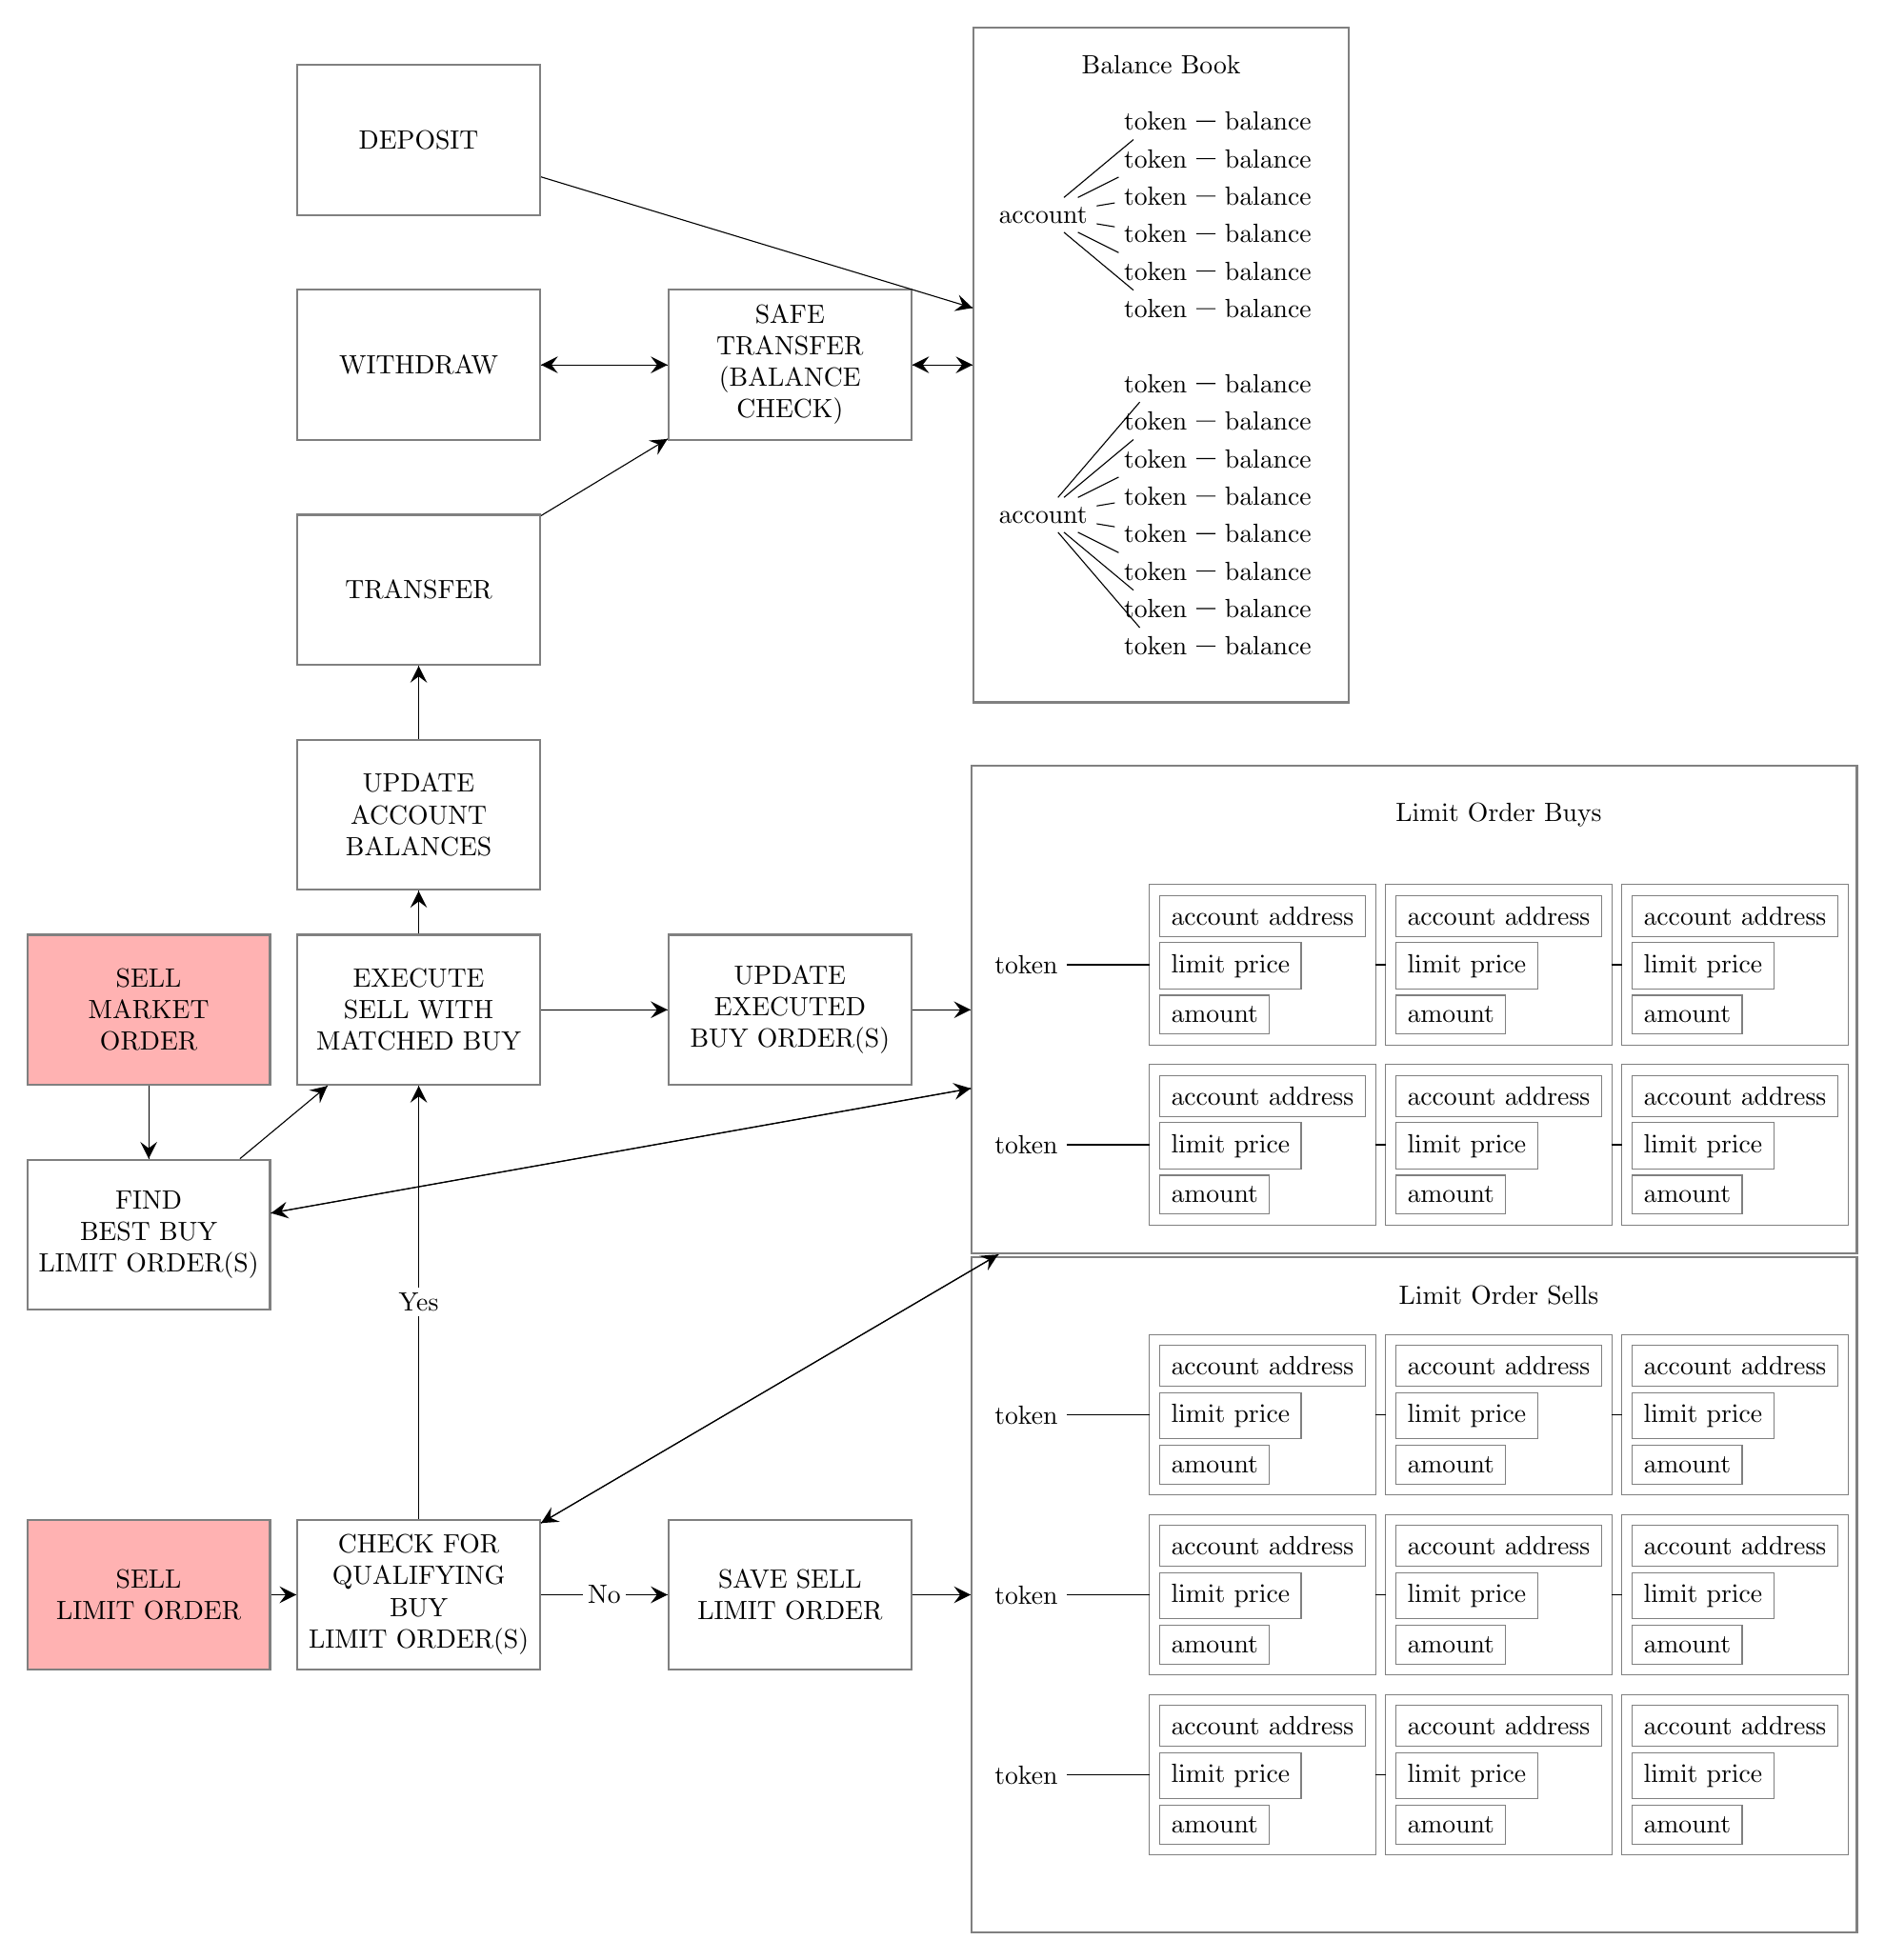
\begin{tikzpicture}[x=4.5cm,y=2cm]
        % Balance Book tree
        \node[style={draw,minimum width=5cm,minimum height=9cm,draw=black!50,thick}] (bbtreeoutline) at (0,0) {};
        \node[style={align=center,text width=3cm,text=black}] (bbtitle) at (0,2) {Balance Book};
        \node (bbtree1) at (-.35,1) {account}[
                grow=east,
                level 1/.style = {sibling distance=.5cm}
            ]
            child {node {token} child {node {balance}} }
            child {node {token} child {node {balance}} }
            child {node {token} child {node {balance}} }
            child {node {token} child {node {balance}} }
            child {node {token} child {node {balance}} }
            child {node {token} child {node {balance}} };
        \node (bbtree2) at (-.35,-1) {account}[
                grow=east,
                level 1/.style = {sibling distance=.5cm}
            ]
            child {node {token} child {node {balance}} }
            child {node {token} child {node {balance}} }
            child {node {token} child {node {balance}} }
            child {node {token} child {node {balance}} }
            child {node {token} child {node {balance}} }
            child {node {token} child {node {balance}} }
            child {node {token} child {node {balance}} }
            child {node {token} child {node {balance}} };
        % Balance Book Functions
        \node[recwht] (bbdeposit1) at (-2.2,1.5) {DEPOSIT};
        \node[recwht] (bbwithdraw1) at (-2.2,0) {WITHDRAW};
        \node[recwht] (bbtransfer1) at (-2.2,-1.5) {TRANSFER};
        \node[recwht] (bbsafetransfer1) at (-1.1,0) {SAFE TRANSFER\\(BALANCE\\CHECK)};

        % Limit Order Buy tree
        \node[style={draw,minimum width=11.8cm,minimum height=6.5cm,draw=black!50,thick}] (lobuyoutline) at (.75,-4.3) {};
        \node[style={align=center,text width=3cm,text=black}] (lobuytitle) at (1,-3) {Limit Order Buys};
        \node (lobuytoken1) at (-.4,-4) {token};
        \matrix[mymatrix] (lobuyt1o1) at (.3,-4) {
            % |[title]|LimitDetail \\
            account address \\
            limit price \\
            amount \\
        };
        \node[mycontainer, fit=(lobuyt1o1)] {};
        \matrix[mymatrix] (lobuyt1o2) at (1,-4) {
            account address \\
            limit price \\
            amount \\
        };
        \node[mycontainer, fit=(lobuyt1o2)] {};
        \matrix[mymatrix] (lobuyt1o3) at (1.7,-4) {
            account address \\
            limit price \\
            amount \\
        };
        \node[mycontainer, fit=(lobuyt1o3)] {};
        \node (lobuytoken2) at (-.4,-5.2    ) {token};
        \matrix[mymatrix] (lobuyt2o1) at (.3,-5.2) {
            account address \\
            limit price \\
            amount \\
        };
        \node[mycontainer, fit=(lobuyt2o1)] {};
        \matrix[mymatrix] (lobuyt2o2) at (1,-5.2) {
            account address \\
            limit price \\
            amount \\
        };
        \node[mycontainer, fit=(lobuyt2o2)] {};
        \matrix[mymatrix] (lobuyt2o3) at (1.7,-5.2) {
            account address \\
            limit price \\
            amount \\
        };
        \node[mycontainer, fit=(lobuyt2o3)] {};

        % Limit Order Sell tree
        \node[style={draw,minimum width=11.8cm,minimum height=9cm,draw=black!50,thick}] (loselloutline) at (.75,-8.2) {};
        \node[style={align=center,text width=3cm,text=black}] (loselltitle) at (1,-6.2) {Limit Order Sells};
        \node (loselltoken1) at (-.4,-7) {token};
        \matrix[mymatrix] (losellt1o1) at (.3,-7) {
            account address \\
            limit price \\
            amount \\
        };
        \node[mycontainer, fit=(losellt1o1)] {};
        \matrix[mymatrix] (losellt1o2) at (1,-7) {
            account address \\
            limit price \\
            amount \\
        };
        \node[mycontainer, fit=(losellt1o2)] {};
        \matrix[mymatrix] (losellt1o3) at (1.7,-7) {
            account address \\
            limit price \\
            amount \\
        };
        \node[mycontainer, fit=(losellt1o3)] {};
        \node (loselltoken2) at (-.4,-8.2) {token};
        \matrix[mymatrix] (losellt2o1) at (.3,-8.2) {
            account address \\
            limit price \\
            amount \\
        };
        \node[mycontainer, fit=(losellt2o1)] {};
        \matrix[mymatrix] (losellt2o2) at (1,-8.2) {
            account address \\
            limit price \\
            amount \\
        };
        \node[mycontainer, fit=(losellt2o2)] {};
        \matrix[mymatrix] (losellt2o3) at (1.7,-8.2) {
            account address \\
            limit price \\
            amount \\
        };
        \node[mycontainer, fit=(losellt2o3)] {};
        \node (loselltoken3) at (-.4,-9.4) {token};
        \matrix[mymatrix] (losellt3o1) at (.3,-9.4) {
            account address \\
            limit price \\
            amount \\
        };
        \node[mycontainer, fit=(losellt3o1)] {};
        \matrix[mymatrix] (losellt3o2) at (1,-9.4) {
            account address \\
            limit price \\
            amount \\
        };
        \node[mycontainer, fit=(losellt3o2)] {};
        \matrix[mymatrix] (losellt3o3) at (1.7,-9.4) {
            account address \\
            limit price \\
            amount \\
        };
        \node[mycontainer, fit=(losellt3o3)] {};

        % Limit Order Actions
        \node[recred] (losell1) at (-3,-8.2) {SELL\\LIMIT ORDER};
        \node[recwht] (lobuycheck1) at (-2.2,-8.2) {CHECK FOR\\QUALIFYING BUY\\LIMIT ORDER(S)};
        \node[recwht] (losellsave1) at (-1.1,-8.2) {SAVE SELL\\LIMIT ORDER};
        \node[recwht] (losellexecute1) at (-2.2,-4.3) {EXECUTE\\SELL WITH\\MATCHED BUY};
        \node[recwht] (lobuyupdate1) at (-1.1,-4.3) {UPDATE\\EXECUTED\\BUY ORDER(S)};
        \node[recwht] (lotransfer) at (-2.2,-3) {UPDATE\\ACCOUNT\\BALANCES};

        \node[recred] (losell2) at (-3,-4.3) {SELL\\MARKET ORDER};
        \node[recwht] (lobuycheck2) at (-3,-5.8) {FIND\\BEST BUY\\LIMIT ORDER(S)};

        \begin{scope} %[every path/.style={-latex}]
            \draw[arrowfwd] (bbdeposit1) -- (bbtreeoutline);
            \draw[arrowfwd] (bbsafetransfer1) -- (bbwithdraw1);
            \draw[arrowfwd] (bbwithdraw1) -- (bbsafetransfer1);
            \draw[arrowfwd] (bbtransfer1) -- (bbsafetransfer1);
            \draw[arrowfwd] (bbsafetransfer1) -- (bbtreeoutline);
            \draw[arrowfwd] (bbtreeoutline) -- (bbsafetransfer1);
            \draw (lobuytoken1) -- (lobuyt1o1);
            \draw (lobuyt1o1) -- (lobuyt1o2);
            \draw (lobuyt1o2) -- (lobuyt1o3);
            \draw (lobuytoken2) -- (lobuyt2o1);
            \draw (lobuyt2o1) -- (lobuyt2o2);
            \draw (lobuyt2o2) -- (lobuyt2o3);
            \draw (loselltoken1) -- (losellt1o1);
            \draw (losellt1o1) -- (losellt1o2);
            \draw (losellt1o2) -- (losellt1o3);
            \draw (loselltoken2) -- (losellt2o1);
            \draw (losellt2o1) -- (losellt2o2);
            \draw (losellt2o2) -- (losellt2o3);
            \draw (loselltoken3) -- (losellt3o1);
            \draw (losellt3o1) -- (losellt3o2);
            \draw[arrowfwd] (losell1) -- (lobuycheck1);
            \draw[arrowfwd] (lobuycheck1) -- (lobuyoutline);
            \draw[arrowfwd] (lobuyoutline) -- (lobuycheck1);
            \draw[arrowfwd] (lobuycheck1) -- node[midway,fill=white,inner sep=2pt] {No} (losellsave1);
            \draw[arrowfwd] (losellsave1) -- (loselloutline);
            \draw[arrowfwd] (lobuycheck1) -- node[midway,fill=white,inner sep=2pt] {Yes} (losellexecute1);
            \draw[arrowfwd] (losellexecute1) -- (lobuyupdate1);
            \draw[arrowfwd] (lobuyupdate1) -- (lobuyoutline);
            \draw[arrowfwd] (losellexecute1) -- (lotransfer);
            \draw[arrowfwd] (lotransfer) -- (bbtransfer1);
            \draw[arrowfwd] (losell2) -- (lobuycheck2);
            \draw[arrowfwd] (lobuycheck2) -- (lobuyoutline);
            \draw[arrowfwd] (lobuyoutline) -- (lobuycheck2);
            \draw[arrowfwd] (lobuycheck2) -- (losellexecute1);
            % \draw (rec3) edge node[midway,fill=white,inner sep=2pt] {No} (cir3);
            % \draw (rec3.north east) -- ++(cir3);
        \end{scope}
    \end{tikzpicture}
\end{document}